The compiler for the \gls{DSL} is implemented in the functional language
Haskell \cite{Haskell}.
Currently, Volr translates its network models into two runtime
environments (backends) based on \gls{OpenCL} through Futhark\index{Futhark} and
\glspl{SNN} simulations through PyNN and NEST.\index{PyNN}\index{NEST}
However, using the learning-to-learn paradigm above, the PyNN implementations
opens for the possibility to transfer the optimised models into neuromorphic
hardware such as BrainScaleS\index{BrainScaleS}.

Futhark was chosen because it is concise and offers
useful abstractions that cleanly compose functional
models \cite{Henriksen2017}.
Considering \glspl{NN} as a structure of feedforward and feedback functions,
Futhark is an elegant solution for the task.

PyNN was chosen for its general purpose API that translates to both, the
neuromorphic BrainScaleS \index{BrainScaleS} backend, as well as the NEST 
\index{NEST} simulator.
\\[0.2cm]
Figure \ref{fig:volr-architecture} shows the workflow starting with the
compilation of the network model, down to the runtime evaluation on each backend.
The following section explains the diagram one component at a time.

\begin{figure}
  \centering
  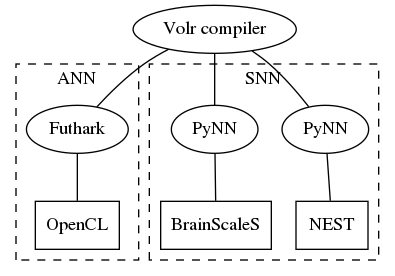
\includegraphics[width=0.6\textwidth]{images/volr-architecture.png}
  \caption{The workflow from the Volr compiler to 
    \gls{ANN} simulations in Futhark or \gls{SNN} simulations in NEST and
    \gls{BrainScaleS}.
  }
  \label{fig:volr-architecture}
\end{figure}

\subsection{The DSL compiler}
The Haskell compiler consists of five different parts:
An \gls{AST}, an evaluator, a language parser and two
code generators for \glspl{ANN} and \glspl{SNN}.

\lstset{mathescape=false,showstringspaces=false}
\begin{minipage}{\linewidth}
  \begin{lstlisting}[language=haskell, caption={The Volr AST in
  Haskell},label={code:term}]
data Term
  = TmNet Int 
  | TmPar Term Term
  | TmSeq Term Term
  | TmRef String
  | TmLet String Term Term
  deriving (Eq, Show)  
\end{lstlisting}
\end{minipage}

The AST reflects the expressions given in the 
specification (see section \ref{sec:volr}) and is
shown in Listing \ref{code:term}.
It is accompanied by a simple type system (in Listing \ref{code:type})
that similarly maps to the types given above.

\begin{lstlisting}[language=haskell,label={code:type},caption={Volr type system
in Haskell}]
data Type 
  = TyNetwork Int Int
  | TyInt
\end{lstlisting}

The evaluator component evaluates the expression tree into
a reference-free model, checking the type integrity in the
process.

Listing \ref{code:eval-type} shows the type checking
that also occurs in the evaluator step. 
If the model is malformed, an error is generated to explain why the
model could not evaluate correctly.
Tests for the type checks and the evaluator are written to ensure the
correctness of the compilation.
They are elaborated in section \ref{sec:verification} on page
\pageref{sec:verification}.

\begin{lstlisting}[language=Haskell,caption={Part of the type checking code in
Haskell.},label={code:eval-type}]
typeOf :: Term -> EvalState Type
typeOf term = 
  case term of
    TmNet n m -> return $ TyNetwork n m
    TmSeq t1 t2 -> do
      leftOut <- sizeRight t1
      rightIn <- sizeLeft t2
      if leftOut == rightIn then do
        leftIn <- sizeLeft t1
        rightOut <- sizeRight t2
        return $ TyNetwork leftIn rightOut
      else
        throwError $ "Type error: Incompatible network sizes. " ++
                     "Output " ++ (show leftOut) ++ " should " ++
                     "be equal to input " ++ (show rightIn)
\end{lstlisting}

The language parser, built with the help of the monadic parser combinator library Megaparsec
\cite{megaparsec}, interprets textual input into the AST. \index{AST}
The main component of the parser is shown in Listing \ref{code:parser}
and the whole parser is available in Appendix \ref{app:implementation} on page
\pageref{app:implementation_parser}.

\begin{lstlisting}[language=Haskell,name=The main component of the text parser
for Volr.,label={code:parser}]
parseTerm :: Parser Term
parseTerm = (lexeme $ choice
  [ TmNet <$> (symbol "Net" *> integer) <*> integer
  , TmPar <$> (symbol "Par" *> (parens parseTerm)) <*> (parens parseTerm)
  , TmSeq <$> (symbol "Seq" *> (parens parseTerm)) <*> (parens parseTerm)
  , TmRef <$> (symbol "Ref" *> (name))
  , TmLet <$> (symbol "Let" *> (name)) <*> (symbol "=" *> parseTerm)
                           <*> (symbol "in" *> parseTerm)
  ]) <* (optional eof)
\end{lstlisting}

Finally two code generators are implemented for the translation into
second and third generation networks.
This translation will be presented along the implementation
for the two backends.

\subsection{Futhark backend} \label{sec:volr-futhark}
This thesis builds on the work by \textcite{Minh2018}, who 
implemented a functional library in Futhark for deep learning.
The library models \gls{NN} layers as records with three fields:
a function for forward propagation, a function for backward propagation
and a cache for weights. 
The backward propagation uses gradient descent to find optimal
weight configurations.
Because of its functional nature, layers can simply be joined 
sequentially by function composition.

The library from \cite{Minh2018} has been modified to fit the
additions in the thesis, and is available online (see links in 
Appendix \ref{app:implementation}).
In particular, a \textit{replicate} and a \textit{merge} layer has
been added, to account for the parallel operator ($\ominus$).
A connection that allows two parallel networks to connect to other
layers has also been added, although it simply composes tuples of
the layer structure (see the file \texttt{neural\_networks.fut} in
Appendix \ref{app:implementation}, page \pageref{app:implementation_fut_nn}).

\paragraph{Replicate layer}
In practice this layer connects to two other networks, and densely
replicates the output to each layer.
This happens by storing two separate collections of weights, such
that each forward connection is assigned the correct value.
Backpropagation works by calculating the error correction on the
two sets of weights. The final error sent to the previous layer
is the average of the error for each neuron. 
The algorithm is shown in a shortened form in Listing \ref{code:bp-replicate}.
Here the two errors and weights are independently calculated.
The weights are stored in the layer as-is, but the errors are 
averaged before they are passed to the previous layer.

\begin{lstlisting}[language=Haskell,label={code:bp-replicate},caption={Part
    of the forward and backward propagation algorithms for the replicate layer.
Abbreviated for clarity.}]
-- Forward propagation
let forward (act:[]t -> []t)
	    (training:bool)
	    ((t1, t2): weights)
	    (input:input) : (cache, output) =
  let feedForward ((w, b): std_weights t): (tup2d t, arr2d t) = [...]
  let (c1, r1) = feedForward t1
  let (c2, r2) = feedForward t2
  in ((c1, c2), (r1, r2))

-- Backward propagation
let backward (act: []t -> []t)
             (first_layer: bool)
             (apply_grads: apply_grad t)
             ((w1, w2): weights)
             ((c1, c2): cache)
             ((e1, e2): error_in) : b_output =
  let (error1, w1) = backProp w1 c1 e1
  let (error2, w2) = backProp w2 c2 e2
  [...]
  in (average_sum_matrix [error1, error2], (w1, w2))
\end{lstlisting}

This interpretation fits with the original specification, after which
the parallel notation duplicates the 'work' in two separate networks.
The complete code for the replication, and the code for translating the \gls{DSL}
abstractions into Futhark,\index{Futhark} is shown in Appendix 
\ref{app:implementation}.

\paragraph{Merge layer}
The merge layer is significantly simpler than the replication layer,
because it merely concatenates the inputs from two parallel layer into one single
layer. 
For that reason it also does not contain any weights.
In the case of backprogapation, the errors are rerouted back to
the population from which the neuron originated.
All optimisation logic is left for the regular dense or replicated
layers.

\begin{lstlisting}[caption={Functions for forward and backward propagation in
the merge layer.}]
-- Forward propagation
let forward  (_:[]t -> []t)
	     (_:bool)
	     (_: weights)
	     ((i1, i2):input) : (cache, output) =
  ((), concat i1 i2)

-- Backward propagation
let backward (_:[]t -> []t) (l1_sz:i32)
	     (_:bool)
	     (_:apply_grad t)
	     (_:weights)
	     (_:cache)
	     (error_concat:error_in) : b_output =
  ((error_concat[0:l1_sz], error_concat[l1_sz:]), ())
\end{lstlisting}

This interpretation is also aligned with the original specification, 
because it allows the parallel populations to propagate their output
independent of each other.

\subsection{PyNN backend}
The interpretation to PyNN\index{PyNN} is done in two steps: a
conversion from the \gls{DSL} into an \gls{SNN} representation,
and a translation between that representation into backend-specific
NEST code in Python. \index{NEST}
The steps are decoupled to enforce the same semantics on the code
generation for the neuromorphic and simulation backends.
While PyNN is designed as a simulator-dependent \gls{API}, 
it is unlikely that the backends will fully support it in the
near future (see section \ref{sec:SNN-simulators}).

\subsubsection{\gls{SNN} translation step}
Before Python code for PyNN can be generated, a number of assumptions
have to be met. 
In particular the types of connections (referred to as projections in PyNN)
and neuron models have to be described with a full set of neuron parameters.
The modelling of this is in Haskell.
The neuron parameters for a LIF\index{LIF} neuron can be seen in Listing
\ref{lst:lif-cond-exp} with their corresponding default values
below\footnote{
The current neuron models and their default parameters are taken from PyNN's
standard models, available at
\url{http://neuralensemble.org/docs/PyNN/standardmodels.html}.
}.

\begin{lstlisting}[language=Haskell,caption={A LIF neuron with exponential decay and
  conductance-based synapses, modelled in Haskell.},label={lst:lif-cond-exp}]
data NeuronType =
    = IFCondExp {
        _v_rest :: Float, -- ^ resting potential
        _cm :: Float, -- ^ membrane capacitance
        _tau_m :: Float, -- ^ membrane time constant
        _tau_refrac :: Float, -- ^ refractory time
        _tau_syn_E :: Float, -- ^ excitatory synaptic time constant
        _tau_syn_I :: Float, -- ^ inhibitory synaptic time constant
        _e_rev_E :: Float, -- ^ excitatory reversal potential
        _e_rev_I :: Float, -- ^ inhibitory reversal potential
        _v_thresh :: Float, -- ^ spike initiation threshold
        _v_reset :: Float, -- ^ reset value for membrane potential after a spike
        _i_offset :: Float -- ^ offset current
    }

if_cond_exp :: NeuronType
if_cond_exp = IFCondExp {
    _v_rest = -65.0,
    _cm = 1.0,
    _tau_m = 20.0,
    _tau_refrac = 0.0,
    _tau_syn_E = 5.0,
    _tau_syn_I = 5.0,
    _e_rev_E = 0.0,
    _e_rev_I = -70.0,
    _v_thresh = -50.0,
    _v_reset = -65.0,
    _i_offset = 0.0
}
\end{lstlisting}

These neuron models form the basis of populations, which is determined by the
neuron model and the number of neurons in the population.
Populations can be understood as neuron groups or nodes in the network graph.
Along spike sources, which generate spikes over time, they are the 
basic components in a spiking neural network graph.
The definition of nodes as populations of neurons are shown in
Listing \ref{lst:node}.

\begin{lstlisting}[language=,caption={The definition of a node as either a population or a
spike source.},label={lst:node}]
data Node = Population {
        _numNeurons :: Integer,
        _neuronType :: NeuronType
    }
\end{lstlisting}

The nodes in the spiking graph are connected through edges shown in 
Listing \ref{lst:projection}.

\begin{lstlisting}[language=,caption={The definition of an edge as a projection between
two nodes with a certain effect.},label={lst:projection}]
data Edge =
      Projection {
          _effect :: ProjectionEffect,
          _input :: Node,
          _output :: Node
\end{lstlisting}

The type of the edges are determined by projection effects, which
in the current implementation is fixed to describe a 
dense projection (\texttt{AllToAll} in PyNN), whose weights are static and
do not change during the simulation.

The model presented here allows to completely reproduce the connection
graph of the \gls{DSL} description.
The only difference between the two is the lack of biases and activation functions
during the feedforward sted in \glspl{SNN}.

\subsubsection{PyNN backend}
The final step in the translation of the \gls{DSL} to PyNN code maps the
\gls{SNN} model from above to executable Python code.
A separate neural network library, VolrPyNN, has been developed for this purpose, and is included in Appendix \ref{app:implementation} on page
\pageref{app:implementation_volrpynn}.
Similarly to the Futhark backend, the Python backend models learning through
backpropagation, but instead of using the traditional feedforward activation
functions, the simulation backend (NEST) is used to generate the spike data.
This requires that the layer knows which derivation function to apply in
the backpropagation step.
To simplify the code, ReLU\index{activation!ReLU} is the default gradient model for all layers.
The Python library also contains the merge, dense,
replicate layer, but because the connections appear through
PyNN\index{PyNN} projections, the parallel layer can be omitted.

Another divergence from the Futhark backend is the normalisation of the
output data through a softmax\index{normalisation!softmax} normalisation
(see Equation \ref{eq:softmax} on page \pageref{eq:softmax}).
This is a commonly used technique for spiking networks to ensure that the 
output stays positive, despite neurons that do not receive any inputs 
\cite{Rueckauer2017}.
This softmax normalisation is only applied in the feedforward step, and does
not interfere with the backpropagation.

The backpropagation algorithm is implemented in the dense layer, and a snippet
is shown in Listing \ref{lst:volrpynn_backprop}.

\begin{lstlisting}[language=Python,label={lst:volrpynn_backprop},caption={Part
of the backpropagation algorithm implemented in PyNN.}]
# Calculate activations for output layer
input_decoded = np.array(self.input_cache)
output_activations = np.matmul(input_decoded, self.weights)

# Calculate output gradients and layer delta
output_gradients = self.gradient_model.prime(output_activations + self.biases)
delta = np.multiply(error, output_gradients)

# Calculate layer backprop and weights, bias updates
backprop = np.matmul(delta, self.weights.T)
weights_delta = np.matmul(input_decoded.T, delta)
(new_weights, new_biases) = optimiser(self.weights, weights_delta,
                                      self.biases, error.sum(axis=0))

self.set_weights(new_weights)
self.biases = new_biases

# Return layer errors
return backprop
\end{lstlisting}

Listing \ref{lst:mnist_pynn} shows an example of the network
\texttt{\textbf{dense} 100 20 $\obar$ \textbf{dense} 20 10}, compiled to a PyNN model in Python.
When activating the input node \texttt{node0} the connections are fed through
the network to the \texttt{node2} output node.
Each projection is initiated with random normal distributed weights, similar
to the Futhark networks.
\ref{app:implementation_volrpynn}.

\begin{lstlisting}[caption={A simple MNIST network in the PyNN backend from the network in figure
    \ref{fig:volr-examples} on page \pageref{fig:volr-examples}.
    The neuron parameters for the LIF populations have been
omitted.},label={lst:mnist_pynn}]
p1 = pynn.Population(100, pynn.IF_cond_exp())
p3 = pynn.Population(20, pynn.IF_cond_exp())
p5 = pynn.Population(10, pynn.IF_cond_exp())
layer0 = v.Dense(p1, p3)
layer1 = v.Dense(p3, p5)
l_decode = v.Decode(p5)
model = v.Model(layer0, layer1, l_decode)
\end{lstlisting}

